\section{Interfaces in materials}

So far we have seen how much important the defects are to describe diffusion inside a solid state system, focussing on how defects allow it in the first place.  Still, we want now to look at a different type of defects that highly influences the diffusion and are \textbf{interfaces}. Basically, real materials are not a simple single block of atoms bonded together, but it's usually composed by chunks of the same material oriented in different directions, called \textbf{grains}, and the regions of space that separate them are the interfaces. We want to look into the description of such objects to see effectively their characteristic and how they influence the diffusion.

At first, we shall say that different types of interfaces exist depending on which type of material separates, like: crystal-vapor, crystal-liquid and crystal-crystal, that are possible to see in \figref{fig:Interfaces}. All of them are interesting and differ not only in the type of phase they connect. For example, it's possible to understand that the local degrees of freedom of such interfaces vary from one to another: in the first two types, in fact, having that liquid and vapor are isotropic then the interface is locally uniquely defined by the normal to the direction in which the interface point, which can be settled by two angles, so two degrees of freedom. On the other side, the crystal-crystal interface is more complex, since we need not only to describe the direction of the cut done by the interface, but also to describe the relative orientation of the two crystals in that position of space. A thing that can be done by imagining the two rotated respect one another, so that we can use the three Euler angle to define it, for a total of 5 degrees of freedom. In our study, we are going to account mainly for a specific type of interface that is defined as follows.
\dfn{Grain boundaries}
{
    A Homophasic interface between crystals with same structure and composition is called grain boundaries.
}
\noindent
Such a defect can be easily seen how describes a specific type of crystal-crystal interface, meaning that we will work in the most complex case with 5 macroscopic variable to work with.

\begin{figure}[b]
    \centering
    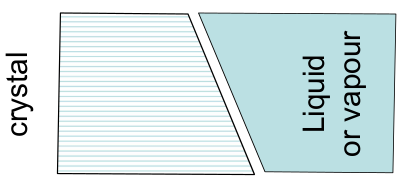
\includegraphics[width=0.4\textwidth]{Immagini/Crys-Liqu.png}
    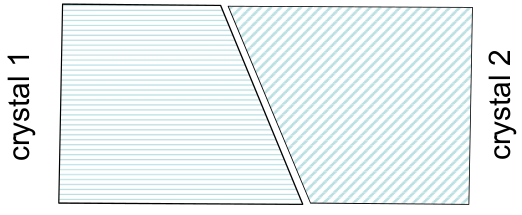
\includegraphics[width=0.4\textwidth]{Immagini/Crys-Crys.png}
    \caption
    {
        Simple image of crystal-liquid/vapor and crystal-crystal interface in order to graphically guide their description of the difference in the degrees of freedom.
    }
    \label{fig:Interfaces}
\end{figure}

Even after this simple description of what an interface is it's already possible to point out why they play a role in diffusive processes. In fact, interfaces can be seen as microscopically as regions of free space inside the material, where the atoms are able to jump from one position to another without the need of breaking bonds with all neighbors or moving all the atoms to pass through. Meaning that, the energy barrier that the processes posses is much lower near such defects, highly boosting the transition rate and, therefore, the diffusivity $D$. Experimental data, shown in \figref{fig:DiffusivityComp}, confirm these simple thoughts showing how the diffusivity of material has a great boost of also several order of magnitudes around interfaces. 
\begin{figure}[t]
    \centering
    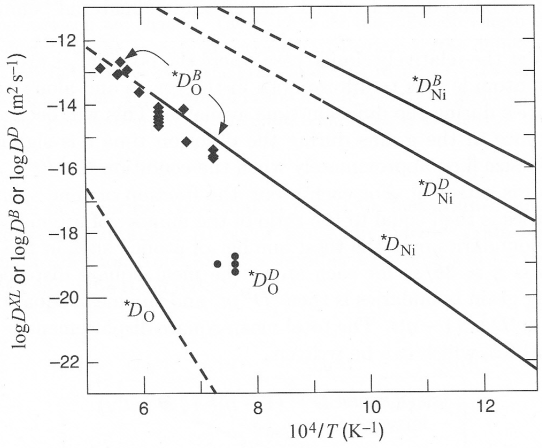
\includegraphics[width=0.4\textwidth]{Immagini/Dbound.png}
    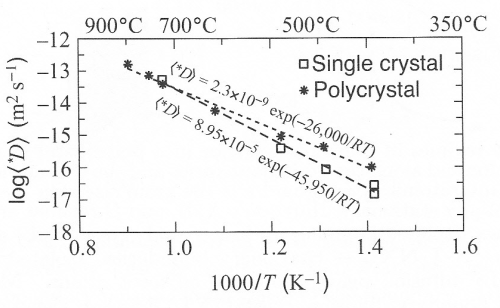
\includegraphics[width=0.55\textwidth]{Immagini/Dmean.png}
    \caption
    {
        Experimental data on the diffusivity value inside \ce{NiO}, with data for pure self-diffusion, $^*D$, diffusion near boundaries, $D^B$, and diffusion near dislocation, $D^D$, on the left. Then, on the right, data on the average value of the diffusivity in a pure single crystal vs a polycrystal which posses interface.
    }
    \label{fig:DiffusivityComp}
\end{figure}
Nevertheless, the average total value of the diffusivity, $D^{eff}$, does not change too much from a single crystal to one composed of grain boundaries and the reason is the following.
\thm{Effective diffusivity}
{
    Inside a polycrystal where the normal diffusivity is $D^{cry}$ and it's value on the boundaries is $D^B$ we will have that the total effective diffusivity is
    \begin{equation}
        D^{eff} = D + \frac{3\delta}{d_G}D^B,
    \end{equation}
    where $d_G$ is the grain size and $\delta$ the boundary thickness.
}
\pf{Proof}
{
    $D^{eff}$ is a weighted average between the pure $D^{cry}$ and $D^B$, where the weights are the relative extent of the volume where the two types of diffusion are active. Meaning that if we account that $V_B \ll V_{cry}$ we can write $V_T \approx V_{cry}$ and the weights are
    \begin{align}
        &w_{cry} = \frac{V_{cry}}{V_{cry}} = 1, &w_B = \frac{V_B}{V_{cry}},
    \end{align}
    where we can think at a grain as a sphere of diameter $d_G$ surrounded by an interface of thickness $\delta$. In this way we can write
    \begin{align}
        &V_B = \pi d_G^2 \delta, &V_{cry} = \frac{\pi}{6}d_G^3,
    \end{align}
    where we shall also take into account that the same interface is shared between two boundaries so that the total weight looks like the following
    \begin{equation}
        w_B = \frac{V_B}{2V_{cry}} = \frac{3\delta}{d_G}.
    \end{equation}
}
\noindent
Basically, due to the much smaller extensions of the interfaces inside the material the average diffusivity changes only partially respect to the incredible increase between $D$ and $D^B$. Still, the result is quite good, especially at lower temperatures since the exponent of $D^B$ is much smaller allowing for an enhancing of the total diffusion by also orders of magnitudes.

By such simple considerations we have already seen how interfaces can be a key point in the description of diffusion inside materials, giving a great boost to the performance overall. For this reason we aim into describing on a more precise level the main properties of such a defect, understanding how they are formed and modelling their evolution.

\nt
{
    Inside the description of surfaces during the course there was also another division between the category of crystal-crystal, defined by the way in which the interfaces are composed. In particular, they are divided between \textbf{sharp}, meaning that atoms form a precise line that divides the two boundaries creating a small interface tens of nanometers long, and \textbf{diffused}, where the interface is not really well-defined since the two phases that is connecting are kind of fused one into the other generating an interface that can be hundreds of nanometers in length.
}

\subsection{Surface free energy}

As in every physical system the best way to see how a system evolve into generating an interface or to see how an interface is structured is to look at the energy. In this case it's easy to understand how creating an interface cost energy, since the creation of grains means that a series of bonds inside the material needs to be broken for the creation of \textbf{surfaces} that delimits the grain boundaries. Therefore, the idea is to focus on the increase of energy counted inside a specific quantity defined as follows.
\dfn{Surface free energy}
{
    We define the surface free energy $\gamma$ as the work needed to create a unit of area inside the wanted material
    \begin{equation}
        \dd w = \gamma \dd A,
    \end{equation}
    where $\dd w$ is the differential of work and $\dd A$ the one of the area.
}
\noindent
Basically, the idea is to compute the total free energy change $\Delta G$ due to interface, which will depend on $\gamma$ along with several factors, and minimize it in order to obtain the form in which such interfaces form inside the material. 

In particular, it's possible to evaluate experimentally or numerically the value of $\gamma$ for several types of interfaces by taking a material separate it and then change the relative angle of orientation between the two pieces. In this way one can find a general increase in the free energy as the angle increase, due to the less coherence between the two parts making the creations of bonds more difficult. Such a phenomenon is well explained inside \figref{fig:Coh-Incoh},
\begin{figure}[t]
    \centering
    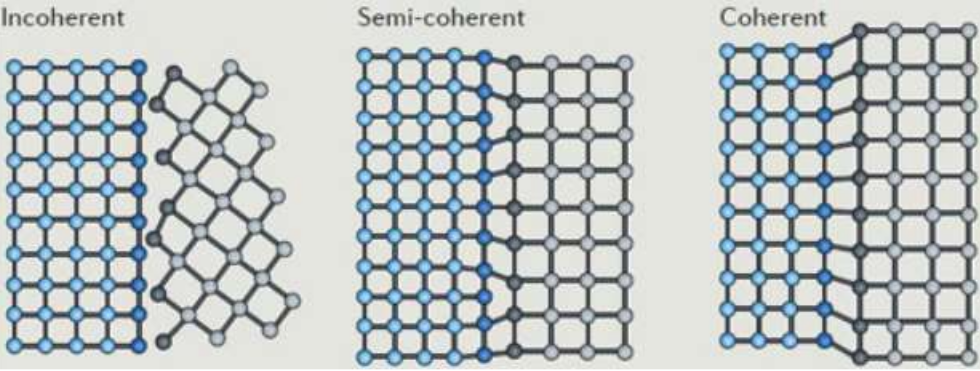
\includegraphics[width=0.8\textwidth]{Immagini/Coh-Incoh.png}
    \caption
    {
        Example of incoherent, coherent and semi-coherent interface, all of them increase the energy of the system but the value of $\gamma$ is lees to the far right and increase going to the left due to the less number of bonds.
    }
    \label{fig:Coh-Incoh}
\end{figure}
where it's possible to see how in the coherent interface the system is only deformed but all the bonds still holds like in the normal crystal minimizing $\gamma$, but maximizing the \textbf{strain energy} $\sigma$. Instead, as we go into the incoherent interface the opposite occur, the system is not deformed but a lot of bonds are broken, maximizing $\gamma$ while minimizing $\sigma$. Therefore, to understand the form that the interface would have in the end we shall minimize the total increase in energy due to its formation keeping in mind that will have a form of the type
\begin{equation}
    \Delta G \approx \gamma A + \sigma V.
\end{equation}
Using it we can understand how the minimization of the energy will bring to a coherent or incoherent interface depending on the extension of the structure variation. Meaning that, if the grain that is formed is small it will have a low $V$ and a larger $A$, bringing to a situation where it's better to minimize $\gamma$ having a coherent interface. While, as the dimensions increase $V$ grows faster respect to $A$ bringing to a preference for incoherent formation minimizing $\sigma$.

Still, this is only an approximation and works only in the contest of tiny grains of particle size, when it comes to describing grain boundaries the volume variation becomes not important due to the fact that the grains are often of similar composition inside the material. This means that in general the main contribution is still given by $\gamma$ inside $\Delta G$ and our main focus will be in minimizing it.

\subsection{Interface motion}

A lot of different internal and external factor can cause interfaces to move or change on a morphological level. For example, the presence of an intrinsic difference in the free energy of the phases that compose the interface, like a crystal-liquid interface where $G_{cry} < G_{liq}$. Leading to an intrinsically lower energy barrier for atoms to hope from liquid to crystal generating a flux of particles. Another possibility is the presence of external stress that generates fluxes of particles inside the material in order to deform it, indirectly changing the grains form and so the interfaces. Still, the main mechanism that we want to discuss here is the one of \textbf{capillary forces} which are forces formed by the presence of $\gamma$ gradients on the interface itself. For example, the presence of two material with different $\gamma$ on a  surface generate a force that tend to mix the two of them in order to smooth $\gamma$ out, a phenomenon called \textbf{Marangoni effect}.

In order to study such a behavior we need to first talk about how to better describe the interface and in particular of the really useful concept of curvature. In particular, we will define the curvature of a surface in a simplified way as follows.
\dfn{Curvature}
{
    Inside a surface, the curvature $\kappa$ in a particular point of the surface is defined as the sum of the curvature on the two main principle axis taken as
    \begin{equation}
        \kappa = \kappa_1 + \kappa_2 = \frac{1}{R_1^c} + \frac{1}{R_2^c},
    \end{equation}
    where $R_i^c$ are the radii of the osculating circles that defines the curvature on the principle axis.
}
\noindent
Such definition allow us to use the curvature inside our computations in order to link two important quantities inside the study of interfaces: area and volume changes. In particular, we can show that the following relation holds.
\begin{figure}[t]
    \centering
    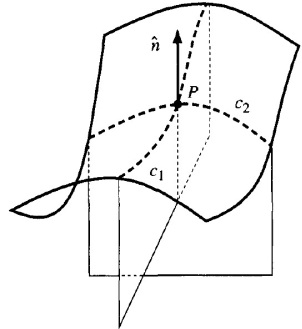
\includegraphics[width=0.3\textwidth]{Immagini/Curv.png}
    \hspace{1cm}
    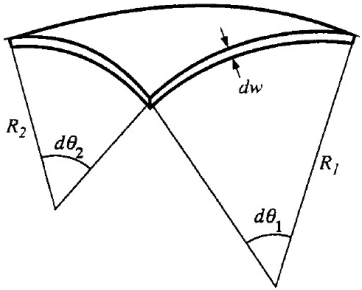
\includegraphics[width=0.4\textwidth]{Immagini/CurvUse.png}
    \caption
    {
        Graphical representation of a generic surface curvature and of the geometrical construction for the connection between the variation of volume and area.
    }
    \label{fig:Curv}
\end{figure}
\thm{Curvature property}
{
    Inside a generic object we can connect the variation of volume to the variation of surface area by the following relation
    \begin{equation}
        \dv{A}{V} = \frac{1}{R_1^c} + \frac{1}{R_2^c} = \kappa.
    \end{equation}
}
\pf{Proof}
{
    We can imagine transforming the variation of volume $\dd V$ in a simple increase of the two osculating radii of a quantity $\dd w$, as shown in \figref{fig:Curv}. In this way we easily write down the variation of area and volume as
    \begin{align}
        &\dd A = \left( R_1 + \dd w \right)\dd \theta_1\left( R_2 + \dd w \right)\dd \theta_2 - R_1\dd \theta_1 R_2\dd \theta_2 = \left( R_1 + R_2 \right)\dd w \dd \theta_1 \dd \theta_2,\\
        &\dd V = R_1\dd \theta_1 R_2 \dd \theta_2\dd w,
    \end{align}
    which can be used to compute the derivative seeing how the wanted relation holds.
}
\noindent
Already, by using such a result, it's possible to see how the increase of energy due to interface expansion can be restated in a more simpler form inquiring volume expansion, like
\begin{equation}
    \dd w = \gamma\dd A = \gamma\kappa\dd V.
\end{equation}
Such a form is also similar to the one of the work done on the mechanical pressure on the system. In fact, at equilibrium the mechanical work $\Delta P \dd V$, where $\Delta P $ is the pressure difference across the interface, needs to be equal to the one done by the surface tension funding out the \textbf{Gibbs-Thomson equation}
\begin{equation}
    \label{eq:Gibbs-Thom}
    \Delta P = \gamma\kappa = \gamma\left( \frac{1}{R_1^c} + \frac{1}{R_2^c} \right).
\end{equation}
This is a great result of classical thermodynamics that is really useful, and from our discussion was obtained really simply. Also, it's possible to understand how in the case we are working with a \textbf{spheric object} $R_1^c = R_2^c$ having $\kappa = 2/R^c$. At last, it's important to keep in mind that in the case we have a hollow inside the material the number of surfaces that increase as the volume changes are two, since the external one expands but also the one inside the hollow. Meaning that for a \textbf{hollow object} the surface tension needs to be multiplied by a factor of $2$.

We want now to focus on a grain boundary surface where no hollow is present and the variation of volumes are created by atoms, or particles, of dimensions $\Omega$ can travel from one point to another through a flux. In this optic we can simply model that flux by setting as driving force the chemical potential biased by the presence of the surface energy as
\begin{equation}
    \label{eq:CurvatureChemPot}
    \Phi = \mu + \gamma\kappa\Omega.
\end{equation}
In this way we can see how an undulating surface will have some positions where the contribution given by $\gamma$ is positive or negative depending on the curvature. Bringing to the creation of a flux of particles that will smooth out the differences in curvature, meaning that the final equilibrium interface will result in a \textbf{smooth surface} with zero $\grad \Phi$. Thus, using some simple considerations we are able to describe really easily surface tension $\gamma$ will act inside the material smoothing the surfaces present in the interfaces, and this is only the beginning. In fact, from \eqref{eq:Gibbs-Thom} we can also grasp how $\gamma$ will also have a role in the description of the pressure around the material, something that can be seen as follows.
\thm{Curvature and vapor pressure}
{
    At equilibrium the vapor pressure around a system depends on both $\gamma$ and $\kappa$ as
    \begin{equation}
        P^{eq}(\kappa) = P^{eq}(0)\exp\left( \frac{\kappa\gamma\Omega}{k_BT} \right).
    \end{equation}
}
\pf{Proof}
{
    We can assume that the chemical potential explicit dependence on the pressure of the material is given by the relation
    \begin{equation}
        \mu(P) = \mu(P^0) + k_BT\ln(P/P^0),
    \end{equation}
    and the potential of the gas phase outside the system is given by $\mu(P^{eq}(\kappa))$, while the one inside it is $\mu(P^{eq}(0)) + \gamma\kappa\Omega$. Meaning that at equilibrium we can set them equal and obtain the wanted relation.
}
\noindent
Basically, not only the curvature generate an atomic flux on the surface to smooth it out, but it also creates a gradient of pressure around the material that generate a flux of gasses particle in the same direction having two concurring mechanisms that smooth out the material. Also, the transport through gasses is much faster for obvious reasons.

Another important consequence that we will need in the next studies is the influence that curvature posses in the composition around a $\beta$ particle immersed in an $\alpha$ matrix. Basically, we can imagine to work inside a system composed by two types of atoms $A$ and $B$ and having a two phase field where grains of $\alpha$ and $\beta$ compositions appear inside the material. We can use an argument analougus to the one of the vapor pressure in order to describe the fraction of $B$ atoms in the $A$-rich $\alpha$ matrix near a $\beta$ grain.
\thm{Curvature and composition}
{
    Around a $B$-rich $\beta$ grain inside an $A$-rich $\alpha$ matrix the equilibrium value of $X_B$ is given by
    \begin{equation}
        \label{eq:EquMolarFracCurva}
        X_B^{eq}(\kappa) = X_B^{eq}(0)\exp\left( \frac{\kappa\gamma\Omega}{k_BT} \right).
    \end{equation}
}
\pf{Proof}
{
    The proof is totally analogous to the one before, only that to describe $\mu$ we need to assume the validity of the Henry's law and write
    \begin{equation}
        \mu_B^\alpha(\kappa) = \mu_B^\alpha(0) + k_BT\ln\left( X_B^{eq}(\kappa)/X_B^{eq}(0) \right),
    \end{equation}
    and then set the equilibrium as
    \begin{equation}
        \mu_B^\alpha(\kappa) - \mu_B^\alpha(0) = \mu_B^\beta(\kappa) - \mu_B^\beta(0) = \kappa\gamma\Omega.
    \end{equation}
}

\noindent
This is a really important result that will play an important role in the description of the coarsening process, as we will see, since will promote the formation of larger grains instead of a lot of smaller ones. In fact the idea is that larger grains have a minor concentration of $B$ atoms around respect to small ones, having that a flux due to concentration gradient is created bringing atoms from smaller grains to larger ones slowly consuming the small in favor of a bigger grain. This also means that in terms of free energy we will have that the smaller grain will have higher values of $\Phi$, since $\kappa$ is greater, as can be seen in \eqref{eq:CurvatureChemPot}. The equilibrium concentration of the $\alpha$ and $\beta$ phases will so change based on the dimensions of the grain, changing also the phase diagram of the grain itself.

\nt
{
    It's interesting to note how the surface tension is also important in the description of capillary effect such as the liquid that naturally rise inside a small tube. Where, after a simple description, it's possible to describe the height of the liquid column through the simple formula
    \begin{displaymath}
        h = \frac{2\gamma\cos\alpha}{\rho g r},
    \end{displaymath}
    where $\alpha$ is the contact angle, $\rho$ the density of the liquid, $\gamma$ the surface tension and $r$ the radius of the capillary. On slides the description is a little more accurate.
}

\subsection{Coarsening of microstructure}

With the study of curvature we have seen how the grains inside the material will evolve in order to minimize $\kappa$ preferring the formation of bigger grains from the slow evaporation of smaller one. This process has a big relevance in the study of material structure and atomic diffusion inside it, and for this reason we want to create a model that allow us to predict how the grains are distributed inside the material. In particular, we will focus on the description of $f(R, t)$ the \textbf{particle size distribution} inside the material, where $R$ will be the grain radius assuming that all of them have a spherical shape.

The idea to model the process is to assume that the material at equilibrium is composed by several spherically shaped grains with composition $\beta$ with an equilibrium concentration of atoms $B$ that depends on their shape as
\begin{equation}
    \label{eq:EquiConc}
    c^{eq}(R) = c^{eq}(\infty) \exp\left( \frac{2\gamma\Omega}{k_BTR} \right) \approx c^{eq}(\infty)\left( 1 + \frac{2\gamma\Omega}{k_BTR} \right).
\end{equation}
Where we have used \eqref{eq:EquMolarFracCurva} substituting the value of the curvature of a sphere $2/R$. Such particles are inside an $\alpha$ matrix that is assumed to have a constant average concentration $\mean{c}$, so that a gradient of concentration appear near every grain since $c$ smoothly change from the average to $c^{eq}(R)$
\begin{equation}
    \grad c \approx \frac{c^{eq}(R) - \mean{c}}{R}\vb{n}.
\end{equation}
Such a gradient generates a flux of $B$ components, $\vb{J} = \tilde{D}\grad c$, that increase or decrease the grain size depending on the size of it. In particular, if the grain is large the equilibrium concentration is smaller bringing material to it, while if $R$ decrease the concentration rise making the $B$ components go away as depicted in \figref{fig:CoarsModel}.
\begin{figure}[t]
    \centering
    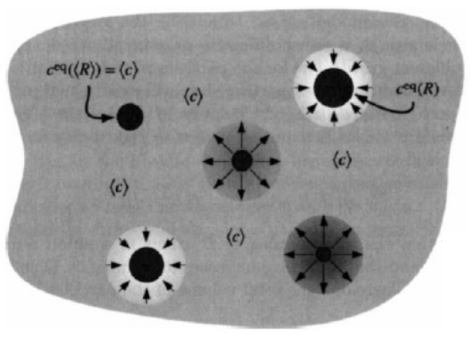
\includegraphics[width=0.6\textwidth]{Immagini/CoarsModel.png}
    \caption
    {
        Model used to describe the coarsening phenomenon inside a material, shows spherical grains inside a uniform concentration matrix where bigger ones attracts atoms while the smaller gave them away.
    }
    \label{fig:CoarsModel}
\end{figure}
Therefore, inside this simple construction we can describe how the grains grows inside the material by describing how the radius evolve over time in the following way
\begin{equation}
    \label{eq:rateOfChange}
    \dv{R}{t} = J\Omega = \tilde{D}\Omega\frac{c^{eq}(R) - \mean{c}}{R}.
\end{equation}
This expression is already interesting, but it's not complete since we don't know how to write down $\mean{c}$. Nevertheless, a form for such an average can be found easily arriving at the following result.
\thm{Growth rate}
{
    Assuming the total volume of the grains is constant the rate of change of the grains sizes takes the following form
    \begin{equation}
        \dv{R}{t} =\frac{2\tilde{D}\gamma\Omega^2c^{eq}(\infty)}{k_B TR}\left( \frac{1}{\mean{R}} - \frac{1}{R} \right).
    \end{equation}
}
\pf{Proof}
{
    If the total volume of the grains remain constant we can write down a simple condition as follows
    \begin{align}
        &\sum_{Grain} R^3 = \text{const}, &\sum_{Grain} R^2\dv{R}{t} = 0.
    \end{align}
    In which we can substitute \eqref{eq:rateOfChange} and using \eqref{eq:EquiConc} inside it we will have
    \begin{equation}
        \sum_{Grain}\tilde{D}\Omega\frac{R^2}{R}\left( \mean{c} - c^{eq}(\infty) - c^{eq}(\infty)\frac{2\gamma\Omega}{k_BTR} \right) = 0.
    \end{equation}
    We can rewrite the expression by manipulating it in the following way
    \begin{equation}
        \left( \sum_{Grain}R \right)\tilde{D}\Omega\left( \mean{c} - c^{eq}(\infty) \right) = \sum_{Grain}c^{eq}(\infty)\frac{2\gamma\Omega}{k_BTR} = N_G c^{eq}(\infty)\frac{2\gamma\Omega}{k_BTR},
    \end{equation}
    then we can then remember how $\mean{R} = \sum_{Grain}R / N_G$ meaning that we simply obtain an evaluation for the average as
    \begin{equation}
        \mean{c} = c^{eq}(\infty)\left( 1 + \frac{2\gamma\Omega}{k_BT\mean{R}} \right).
    \end{equation}
    Substituting it inside the expression of $\dd R/\dd t$ gets us the wanted result.
}
\begin{figure}[t]
    \centering
    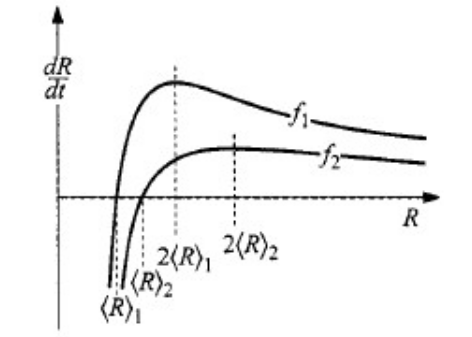
\includegraphics[width=0.4\textwidth]{Immagini/RateGrowth.png}
    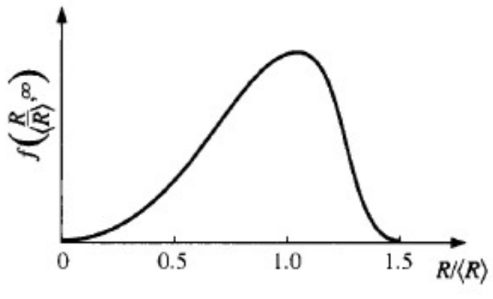
\includegraphics[width=0.45\textwidth]{Immagini/RDistr.png}
    \caption
    {
        Graph of the rate of growth of the grains inside the GLSW theory as a function of the particle size for two different types of grains, on the left. A graph of the solution of the continuity equation for the size distribution at equilibrium on the right.
    }
    \label{fig:rateRdist}
\end{figure}

\noindent
This equation shows to us quantitatively when the grains will start to increase or decrease in size, seeing how they increase when $R > \mean{R}$ and vice versa. Also, if we plot it, as in \figref{fig:rateRdist}, we can see how it's form has a maximum for every grain type that is reached at $R = 2\mean{R}$ and then reaches a plateau as the dimensions grows further.

At last, we shall describe how to work out a form for $f(R, t)$ and in order to do that we can still focus on the fact that the number of particle inside the system needs to be conserved. Meaning that the volume of the grains has to be conserved in the structure having that the continuity equation can be written out having
\begin{equation}
    \label{eq:DistEvo}
    \pdv{f}{t} = -\pdv{J}{R} = -\pdv{}{R}\left[ f(R,t)\pdv{R}{t} \right].
\end{equation}
Where we have used the definition of flux as $\vb{J} = n\vb{v}$ with $n$ the density of material and $\vb{v}$ the average velocity, in our case the density is the distribution of grains volume and the velocity the growth rate. Such an equation allow us to know how the distribution evolves over time, meaning that the initial form of $f(R, 0)$ can be taken as wanted and then evolves following \eqref{eq:DistEvo} since it goes into equilibrium. An example of this is shown in \figref{fig:rateRdist} where the equilibrium form of $f$ is shown for a starting configuration given by a Gaussian. The latter shows how the most probable dimension of a grain is $1.13\mean{R}$ with a cut-off radius of $R_{co} = 1.5\mean{R}$ after which no grains are presents. That distribution also allows us to describe the evolution of the front over time, meaning that in time $R_{co}$ evolves, and we can see how such evolution goes on as follows.
\thm{Cut-off radius growth}
{
    The biggest possible size of grains inside a material grows with time following the simple equation
    \begin{equation}
        \label{eq:cutoffGrowth}
        \mean{R(t)}^3 - \mean{R(0)}^3 = \frac{8\tilde{D}\gamma\Omega^2c^{eq}(\infty)}{9k_BT}t = K_Dt.
    \end{equation}
}
\pf{Proof}
{
    Taking the distribution in \figref{fig:rateRdist} it's possible to take the average of the size as $2R_{co}/3$ so that we can write down
    \begin{equation}
        \eval{\dv{R}{t}}_{R=R_{co}} = \frac{2\tilde{D}\gamma\Omega^2c^{eq}(\infty)}{k_BTR_{co}}\left( \frac{3}{2R_{co}} - \frac{1}{R_{co}} \right) = \frac{\tilde{D}\gamma\Omega^2c^{eq}(\infty)}{k_BTR_{co}^2}.
    \end{equation}
    Then, we can take $R_{co}^3$ and take it's derivative to obtain the value
    \begin{equation}
        \dv{R_{co}^3}{t} = R^2_{co} \eval{\dv{R}{t}}_{R=R_{co}} = \frac{\tilde{D}\gamma\Omega^2c^{eq}(\infty)}{k_BT},
    \end{equation} 
    which can be integrated obtaining a form for the wanted value which then needs to be averaged over the $f$ distribution to obtain the final result.
}
\noindent
This is the final result for this model for the coarsening or \textbf{Ostwald ripening} phenomenon in the contest of \textbf{Greenwood-Lifshitz-Slyozov-Wagner theory}, which is a diffusion limited theory. Meaning that all the velocity at which the grains' growth is dictated by the diffusion velocity inside the matrix. It's also possible to take into account a situation where diffusion in the matrix is really fast and the slow step is the transfer of material inside and outside the grains across the interface. This case is called source limited, the concentration of the matrix is really uniform thanks to fast diffusion, and \eqref{eq:cutoffGrowth} can be rewritten as
\begin{equation}
    \mean{R(t)}^2 - \mean{R(0)}^2 = K_St.
\end{equation}
\nt
{
    Just a little notice, during the lecture another really cool effect was just introduced called \textbf{Rayleigh instability}, which describes how a wire tend to not be stable as the temperatures rise up, or the thickness goes down. Basically, if I take a gold nanowire with a certain thickness we have a certain temperature after which will start to ripe and transform in a series of nanosphere with a certain spacial ordering given by $\lambda$. Also, the ripening temperature goes down as the thickness goes down having that a copper nanowire with \SI{30}{\nano\metre} in diameter will be completely formed by spheres at \SI{400}{\degreeCelsius} but a \SI{40}{\nano\metre} one not.
}